
%(BEGIN_QUESTION)
% Copyright 2011, Tony R. Kuphaldt, released under the Creative Commons Attribution License (v 1.0)
% This means you may do almost anything with this work of mine, so long as you give me proper credit

This P\&ID shows an incinerator stack used to safely burn poisonous gases.  The high temperature of the gas flame reduces the poisonous compounds to relatively harmless water vapor, carbon dioxide, and oxides of sulfur and nitrogen:

$$\includegraphics[width=15.5cm]{i0004rx01.eps}$$

Identify where the measurement/control system is performing {\it integration} to ``totalize'' a quantity over time.  If possible, identify realistic units of measurement for the integrated value(s).

\vskip 10pt

Suppose an environmental regulatory agency required that the emissions monitoring system (loop number 33 in the P\&ID) calculate the {\it total volume} of pollutants emitted each month, rather than just provide measurements of pollutant concentration (e.g. percent or parts-per-million).  How would it be possible to do this, and what additional field instrumentation would be required?

\underbar{file i03507}
%(END_QUESTION)





%(BEGIN_ANSWER)

FIQ-38 is a mass flow totalizer, integrating the mass {\it flow rate} signal coming from flow transmitter FT-38 to arrive at a total mass of fuel gas burned over time.  Realistic units of measurement would be kilograms or pounds (mass).

\vskip 10pt

In order to do the same for stack emissions, we would need to measure the flow rate of exhaust through the incinerator stack, then multiply that flow rate signal by each pollutant's measured concentration (to arrive at flow rate for each pollutant), then integrate each of those pollutant gas flow rates over time to calculate pollutant volumes.

%(END_ANSWER)





%(BEGIN_NOTES)

\vskip 20pt \vbox{\hrule \hbox{\strut \vrule{} {\bf Virtual Troubleshooting} \vrule} \hrule}

This question is a good candidate for a ``Virtual Troubleshooting'' exercise.  Presenting the diagram to students, you first imagine in your own mind a particular fault in the system.  Then, you present one or more symptoms of that fault (something noticeable by an operator or other user of the system).  Students then propose various diagnostic tests to perform on this system to identify the nature and location of the fault, as though they were technicians trying to troubleshoot the problem.  Your job is to tell them what the result(s) would be for each of the proposed diagnostic tests, documenting those results where all the students can see.

During and after the exercise, it is good to ask students follow-up questions such as:

\begin{itemize}
\item{} What does the result of the last diagnostic test tell you about the fault?
\item{} Suppose the results of the last diagnostic test were different.  What then would that result tell you about the fault?
\item{} Is the last diagnostic test the best one we could do?
\item{} What would be the ideal order of tests, to diagnose the problem in as few steps as possible?
\end{itemize}

%INDEX% Basics, control loop troubleshooting (realistic P&ID shown)
%INDEX% Control, strategies: cascade (realistic P&ID shown)
%INDEX% Fieldbus, HART: multivariable instrument (realistic P&ID shown)
%INDEX% Process: incinerator (realistic P&ID shown)

%(END_NOTES)

